\begin{frame}{Neural Network considered}
    \vspace{-2pt}
    We consider a parametric NN with 4 inputs and 4 outputs, defined by
    $$U_\theta(\bm{x},\bm{\mu}) = \big(u_\theta,v_\theta,p_\theta,T_\theta)(\bm{x},\bm{\mu}).$$
    
    The Dirichlet boundary conditions are imposed on the outputs of the MLP by a \textbf{post-processing} step. \citep{Sukumar_2022}
    
    \begin{center}
        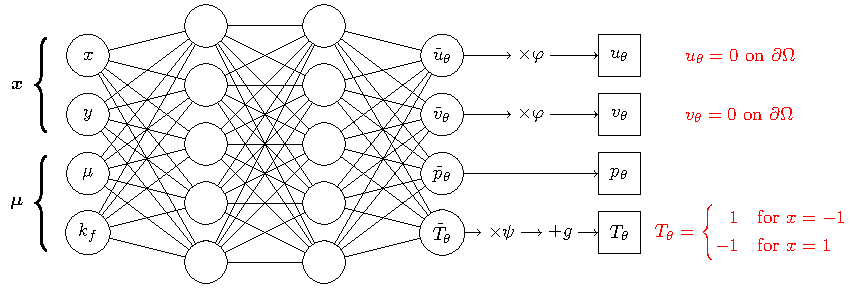
\includegraphics[width=0.74\linewidth]{images/pinn/network/network.pdf}
    \end{center}
    We consider two levelsets functions $\varphi_1$ and $\varphi_2$, and the linear function $g$ defined by
    \begin{equation*}
        \varphi_1(x,y) = (x-1)(x+1)(y-1)(y+1),
    \end{equation*}
    \begin{equation*}
        \varphi_2(x,y) = (x-1)(x+1) \quad \text{and} \quad g(x,y) = 1 - (x+1).
    \end{equation*}
\end{frame}

\begin{frame}{PINN training}
    \vspace{-4pt}
    \textbf{Approximate the solution of \eqref{eq:Pb} by a PINN :} Find the optimal weights $\theta^\star$, such that
	
    \vspace{-8pt}
    \begin{equation}
		\label{eq:opt_pb}
		\theta^\star = \argmin_{\theta}	\big( J_{inc}(\theta) + J_{mom}(\theta) + J_{ener}(\theta) + J_{ad}(\theta) \big),
		\tag{$\mathcal{P}_\theta$}
	\end{equation}

    \vspace{-2pt}
	where the different cost functions\footnote[frame,1]{Discretized by a random process using Monte-Carlo method.} are defined by
	\vspace{5pt}

	\begin{minipage}{0.24\linewidth}
		\centering
		\textcolor{red}{adiabatic condition}
        
		\vspace{12pt}
		\textcolor{orange}{$3$ residual losses}
	\end{minipage}
	\begin{minipage}{0.68\linewidth}
		\centering
        \fcolorbox{red}{white}{
            $J_{ad}(\theta) =
            \int_{\mathcal{M}}\int_{\partial \Omega\vert_{y=\pm 1}} \big| \frac{\partial T_\theta(\bm{x},\bm{\mu})}{\partial n} \big|^2 d\bm{x} d\bm{\mu},$}
        
        \vspace{3pt}
		\fcolorbox{orange}{white}{
            $J_{\textbullet}(\theta) =
                \int_{\mathcal{M}}\int_{\Omega}
                \big| R_{\textbullet}(U_\theta(\bm{x},\bm{\mu});\bm{x},\bm{\mu}) \big|^2 d\bm{x} d\bm{\mu},$}
	\end{minipage}
    
    \vspace{5pt}
    with $U_\theta$ the parametric NN and $\textbullet$ the PDE considered (i.e. $inc$, $mom$ or $ener$).

    %\footnote[frame,2]{We consider a MLP with 5 hidden layers ($40,60,60,60,40$) and a 'sine' activation function. We train the PINN over $10000$ epochs ($3000$ ADAM / $7000$ LBFGS) with $40000$ collocation points in $\Omega$ and $30000$ points on the boundary $\partial\Omega\vert_{y=\pm 1}$.}
    
    \vspace{3pt}    
    \begin{center}
        \begin{minipage}{0.72\linewidth}
            \centering\footnotesize
            \begin{table}[htbp]
                \centering
                \begin{tabular}{cc}
                    \toprule
                    \multicolumn{2}{c}{\textbf{Network - MLP}} \\
                    \midrule
                    \textit{layers} & $40,60,60,60,40$ \\
                    \cmidrule(lr){1-2}
                    $\sigma$ & sine \\
                    \bottomrule
                \end{tabular}
                \hspace{0.1cm}
                \begin{tabular}{cccc}
                    \toprule
                    \multicolumn{4}{c}{\textbf{Training} (ADAM / LBFGs)} \\
                    \midrule
                    \textit{lr} & 7e-3 & \textcolor{red}{$N_\text{col}$} & 40000 \\
                    \cmidrule(lr){1-2} \cmidrule(lr){3-4}
                    $n_{epochs}$ & 10000 & \textcolor{orange}{$N_\text{bc}$} & 30000 \\
                    \bottomrule
                \end{tabular}
            \end{table}

        \end{minipage}
        \begin{minipage}{0.26\linewidth}
            \centering
            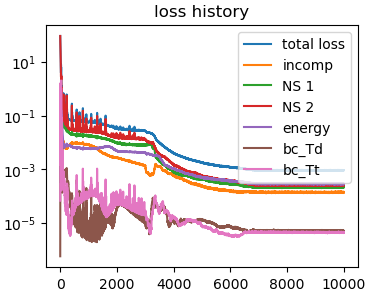
\includegraphics[width=\linewidth]{images/pinn/training/test4_v5.png}
        \end{minipage}
    \end{center}
    
    \vspace{-5pt}
\end{frame}

\begin{frame}{PINN solution}
    % TODO (entrainement + solution pour 1 paramètre ?)
    \vspace{-5pt}
    \begin{center}
        $\bm{\mu}^{(1)} = (0.1,0.1), \; \bm{\mu}^{(2)} = (0.05,0.05) \; \text{and} \;$\fcolorbox{red}{white}{$\bm{\mu}^{(3)} = (0.01,0.01)$}

        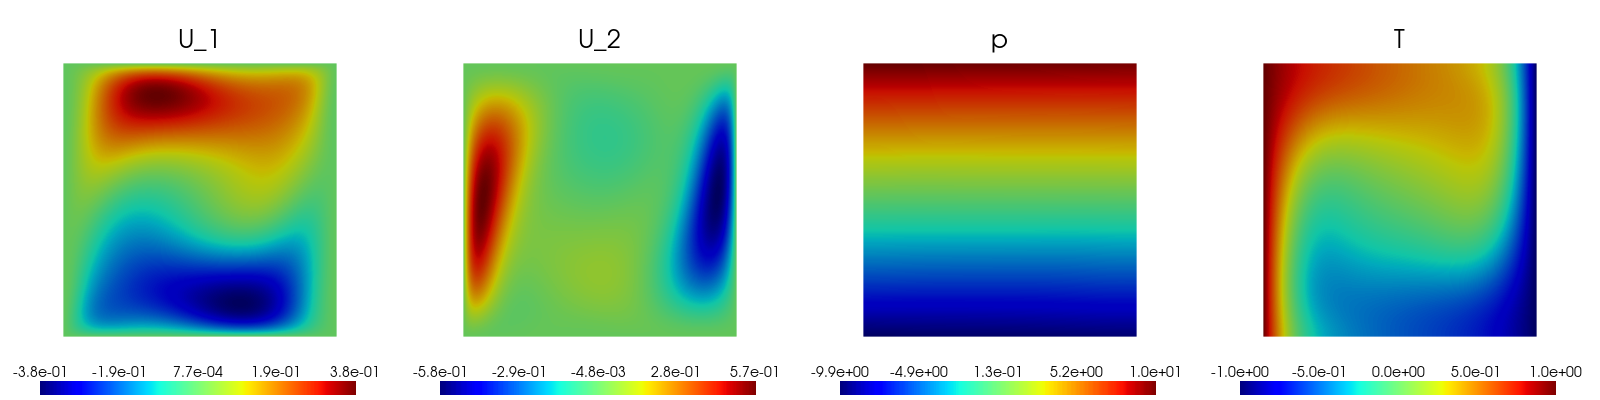
\includegraphics[width=\linewidth]{images/pinn/training/PINN_plot_case4_v5_param3.png}
        
        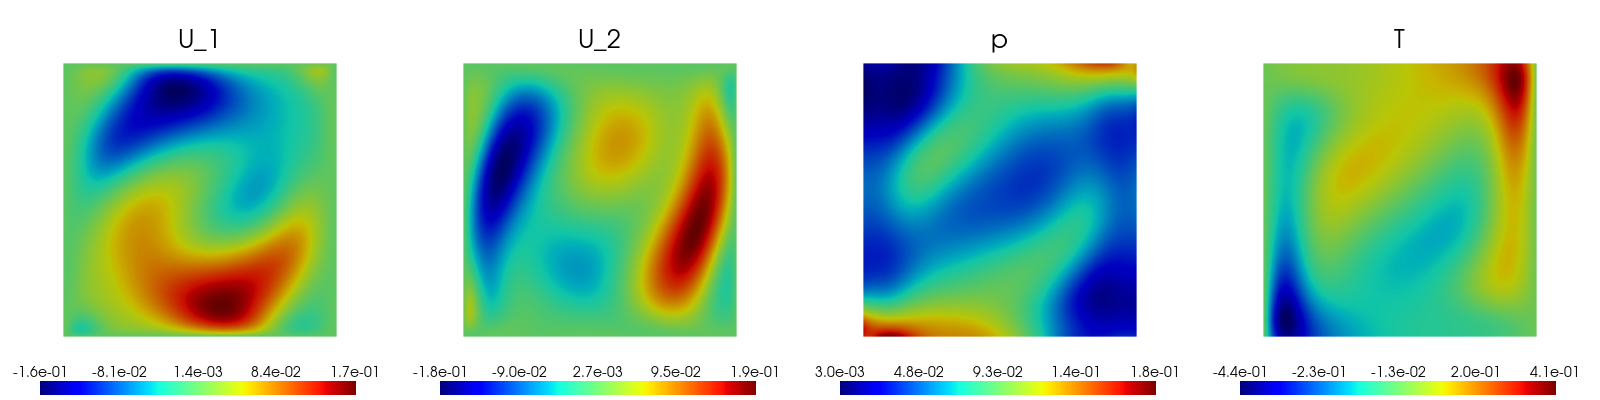
\includegraphics[width=\linewidth]{images/pinn/training/PINN_error_plot_case4_v5_param3.png}
    \end{center}

    \hl{TODO : renommer figure $u_\theta\dots$ (solutions et erreurs) + ajouter erreurs L2}

\end{frame}